
\chapter{Arrival time prediction for journey planning}
\label{cha:etas}

Arrival time prediction is most often used to provide commuters with a countdown while they wait for their bus, and has been shown to reduce experienced wait time \citep{cn}. However, research as also shown that \gls{rti} allows passengers the ability to plan their arrival at a bus stop, resulting in shorter \emph{actual} wait times \citep{cn}. This demonstrates that, if reliable, passengers are likely to make use of \gls{rti} to better plan their commutes. In this chapter, we shift our focus from the probabilistic view of arrival time estimation in \cref{cha:prediction} to a practive one.


Accurately predicting the arrival time of a transit vehicle is a decidedly difficult problem. There are several known sources of variability---traffic lights and intermediate bus stops, for example---but also countless others which we cannot model. \citet{Mazloumi_2011} demonstrated the use of prediction intervals, but the focus was for operations management (TOM\footnote{confirm this}) rather than \gls{rti} for passengers. More recently, \citet{Fernandes_2018} investigated uncertainty displays using quantile dotplots, and found good evidence to suggest that commuters were able to make use of this additional information (TOM\footnote{rewrite this more accurately according to what the paper actually did}). We will examine the use of a single point estimate in an attempt to balance reliability and accuracy and compare this with the use of an interval estimate to convey uncertainty. Our results are based purely on outcome probabilities, however, and not passenger surveys.


Another important aspect of \gls{rti} is journey planning: given an origin and a destination, and optionally one or more constraints---arrive by a certain time, for example---what is the optimal route (or routes for journeys requiring mutliple \emph{legs}). \Citet{Berczi_2017} developed an approach to journey planning that uses a \emph{probabilistic model} of arrival times to decide between competing options. Since the initial selection of candidate options is a complicated topic (see \citet{Hame_2013a,Hame_2013b,Zheng_2016} for methods of doing so) we do not consider this problem in this work. Instead, we use our results to decide between pre-defined options.


Both the arrival time estimates (point and interval) and journey planning decisions use the arrival time distribution estimated in chapter 5. First, however, we need to express the distribution of arrival times in a form we can easily work with (and export from the real-time application). The first consideration is that \glspl{eta} are typically displayed as integers, so we need to decide how to round values. For example, 105~seconds is 1.75~minutes: should this be displayed as 2~minutes (standard rounding) or 1~minute (round down)?


We use Bayesian posterior predictive probabilities, and may want to estimate the median such that $\Pr{A \geq a} = 0.5$; however, if we round $a$ in the above example to 2 minutes, then the equality is incorrect: the probability that the actual arrival time $A$ is later than the estimated arrival time $a$ is \emph{less} than 0.5. Therefore, we find the maximum integer value of $a \in \{0, 1, 2, \ldots\}$ such that $\Pr{A \geq a} \geq 0.5$.


To compute the \gls{cdf} of integer-valued arrival times, we first convert each particle's arrival time $\Tarr\vi$ to minutes and round down, which is the equivalent of taking its modulus with 60:
\begin{equation}
\label{eq:particle_eta_modulus}
\breve\Tarr\vi = \Tarr\vi \mod 60.
\end{equation}
Next we tally the number of particles with each arrival times $a$ and calculate the probability of the bus arriving in the interval $[a,a+1)$:
\begin{equation}
\label{eq:pf_pdf_arrivaltime}
\Pr{A \in [a, a+1)} =
\frac{1}{N^\star} I_{\breve\Tarr\vi = a}
\end{equation}
where $I_{a=b}$, the indicator, is 1 if $a$ equals $b$, or zero otherwise. Computationally, this is significantly easier than computing quantiles, since the latter involves sorting the particles (see \cref{app:particle-summaries}), whereas tallying integers can be performed with a single, unsorted pass over the particles.


By using \cref{eq:pf_pdf_arrivaltime}, we can express the \gls{cdf} as
\begin{equation}
\label{eq:pf_pdf_arrivaltime}
\Pr{A < a} = \sum_{x=0}^{x=a-1} \Pr{A \in [x, x+1)}.
\end{equation}
\Cref{fig:eta_cdf} presents the \gls{cdf} for a single stop. The remainder of this chapter explores choices of summary statistics to convey this distribution to commuters.


\begin{knitrout}\small
\definecolor{shadecolor}{rgb}{0.969, 0.969, 0.969}\color{fgcolor}\begin{figure}

{\centering 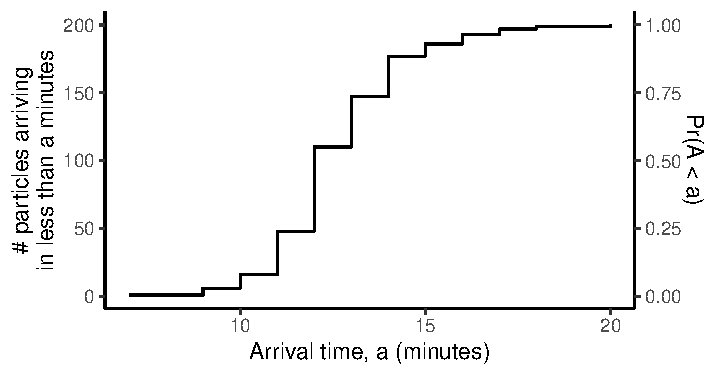
\includegraphics[width=.6\textwidth]{figure/eta_cdf-1} 

}

\caption[CDF of arrival time]{CDF of arrival time.}\label{fig:eta_cdf}
\end{figure}


\end{knitrout}



\section{Estimates of arrival time}
\label{sec:eta_estimates}

As previously discussed, there is considerable uncertainty in the posterior predictive distribution of arrival time. This uncertainty makes point estimates challenging to provide since there is a strong negative correlation between \emph{accuracy}---how far the estimates are from the actual value---and \emph{reliability}---how \emph{useful} the estimate is. Take, for example, the median, which has, in theory, the best accuracy, but 50\% of the time the bus arrives earlier than it predicts, which could result in a passenger missing their bus were they to arrive at the predicted time. An alternative to using point estimates that allows conveyance of uncertainty is to use \emph{prediction intervals}.

The method for obtaining estimates from the \glspl{cdf} from \cref{eq:pf_pdf_arrivaltime} uses quantiles, such that the $q$-quantile, $q\in(0,1)$, is obtained by solving
\begin{equation}
\label{eq:eta_calc_quantile}
\hat\Teta_q = \max\left\{a \in \{0, 1, \ldots\} : \Pr{A < a} \leq q\right\}
\end{equation}
\Cref{fig:eta_calc_quantile} shows a single \gls{cdf} with a horizontal line at $q = 0.5$, where the solution to \cref{eq:eta_calc_quantile} is the maximum of the values below this line (the red points) which is, in this case, $\hat\Teta_{0.5} = 11$.


\begin{knitrout}\small
\definecolor{shadecolor}{rgb}{0.969, 0.969, 0.969}\color{fgcolor}\begin{figure}

{\centering 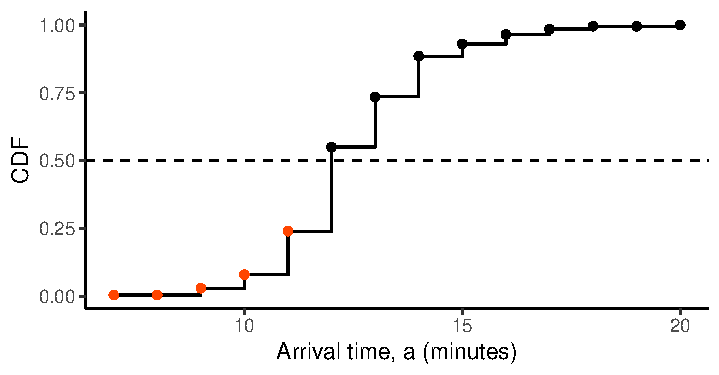
\includegraphics[width=.6\textwidth]{figure/eta_calc_quantile-1} 

}

\caption[Quantile estimation from a CDF]{Quantile estimation from a CDF. ETA values with quantiles below the desired threshold (0.5) are coloured red; the maximum of these is the desired quantile value.}\label{fig:eta_calc_quantile}
\end{figure}


\end{knitrout}


\subsection{Point estimate}
\label{sec:etas-point}

In a perfect world, it would be possible to predict precisely how long it would take a bus to arrive at a stop, and display this single number to passengers. Alas, as we saw in \cref{cha:prediction}, this is not a perfect world, and arrival time prediction inherently comes with significant uncertainty. Yet we still need to decide on the best single value to use as a point estimate of arrival time, since much of the infrastructure currently available only allows this. We also want to examine if it is possible to come up with a single statistic that performs well---on average---and, more importantly, better than the currently deployed method.





\begin{knitrout}\small
\definecolor{shadecolor}{rgb}{0.969, 0.969, 0.969}\color{fgcolor}\begin{figure}

{\centering 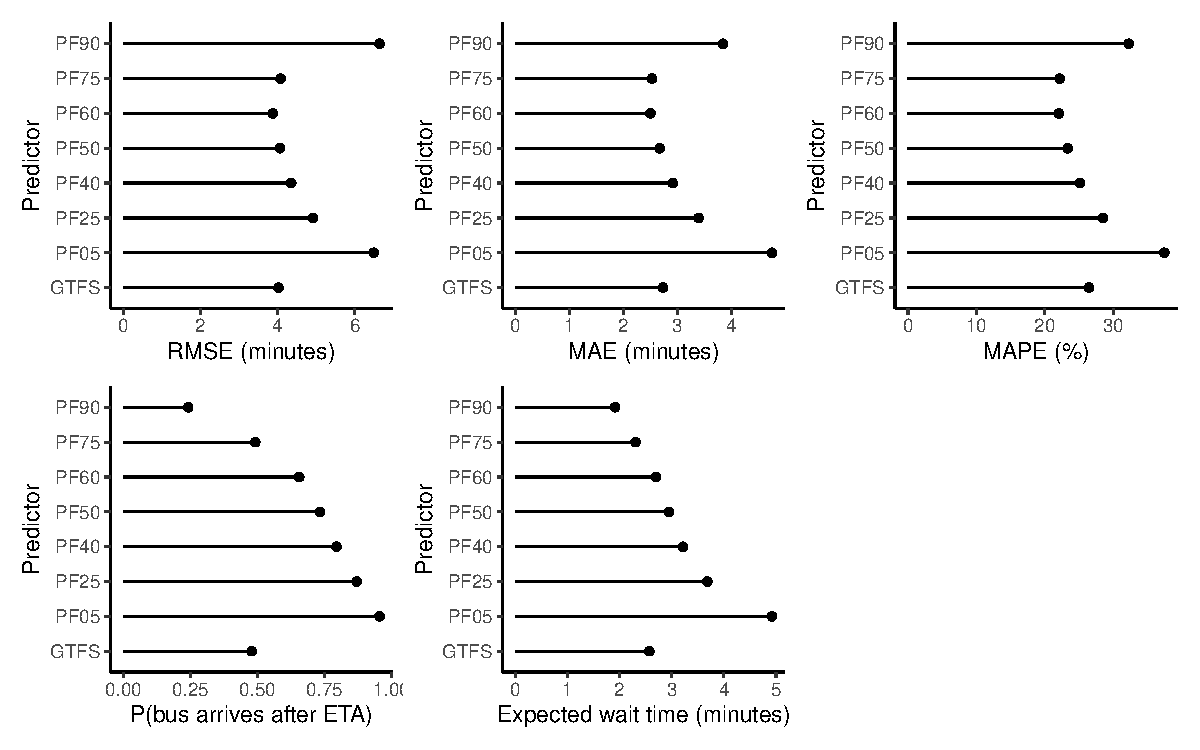
\includegraphics[width=\textwidth]{figure/eta_overall_results-1} 

}

\caption[Comparison of summary statistics for various quantiles of the predictive distribution, and the currently deployed GTFS method]{Comparison of summary statistics for various quantiles of the predictive distribution, and the currently deployed GTFS method. Results are displayed for all day average, and off-peak (between 9h30 and 14h30).}\label{fig:eta_overall_results}
\end{figure}


\end{knitrout}


We calculated, for all stops, trips, and times, a range of arrival times quantiles ($q \in \{0.05, 0.25, 0.5, 0.6, 0.6, 0.75, 0.9\}$), and for each computed the \gls{rmse}, the probability of catching the bus given you arrive at the stated \gls{eta}, $\Pcatch$, and the expected waiting time given you catch the bus, $\Ewait$. The results are displayed in \cref{fig:eta_overall_results}, along with the same values computed used the \gls{gtfs} arrival time estimates. For the particle filter, the lowest \gls{rmse} value is achieved when using the 60\% quantile, which obtains a 67\% probability of the bus arriving after the \gls{eta} and an expected waiting time of 2.7~minutes. The coverage of the quantiles are being overestimated---we would expect the 60\% quantile to have an approximately 40\% success rate---which indicates that the current implementation of the particle filter is underestimating arrival times.


\begin{knitrout}\small
\definecolor{shadecolor}{rgb}{0.969, 0.969, 0.969}\color{fgcolor}\begin{kframe}


{\ttfamily\noindent\bfseries\color{errorcolor}{\#\# Error in eval(lhs, parent, parent): object 'c05' not found}}\end{kframe}
\end{knitrout}

An important consideration is the cost of missing the bus. For each trip, we computed the scheduled time between the current trip and the subsequent one (which is termed \emph{headway}) to compute the expected waiting time if the bus arrives \emph{before} the predicted time. That is, if a bus is predicted to arrive in 5~minutes, but actually arrives in 3, and the time until the next bus (servicing the same trip) is 10~minutes, then the expected waiting time will be $10-5=5$~minutes (assuming the passenger arrives in 5~minutes). This \emph{headway} is an essential component to prediction cost.

The total expected wait time can be conditioned on whether or not the bus was caught,
\begin{equation}
\label{eq:eta_wait_conditional}
\begin{split}
\E{\text{wait}} &=
  \Pr{\text{catch}} \E{\text{wait}|\text{catch}} +
  (1 - \Pr{\text{catch}}) \E{\text{wait}|\text{miss}} \\
  &= \Pr{A \geq a} \E{A - a | A \geq a} +
  \Pr{A < a}\E{\text{headway} - a + A | A < a}
\end{split}
\end{equation}
where $a$ is the estimated arrival time, and $A$ is the actual. For simplicity, we assume headway is maintained (which it is not, \citet{})---that is, if a bus has 20~minute frequency and you miss the bus by 5~minutes, your expected waiting time is 15~minutes.

\Cref{fig:eta_headway_results} shows the values of $\Pcatch$, $\Ecatch$, $\Emiss$, and $\Ewait$ by headway (rounded down, in minutes). Capture probability is not so affected by headway, though it decreases slightly for longer headways. In contrast, expected wait times are very much affected. Most unexpectedly, $\Ecatch$ decreases with headway, which could be caused by a higher proportion of short headway at peak times when traffic is more congested, leading to more uncertainty (so the quantiles are more dispersed), or the buses take longer than expected. For $\Emiss$, the expected wait time is not unexpectedly strongly correlated with headway. Overall, the difference in $\Ewait$ between predictors is negligible for headways less than 10~minutes, after which time differences appear. Low frequency routes should prefer a low quantile to reduce the chance of missing the bus.


We did not examine time-until-arrival, which we saw in the previous chapter explained a lot of the variation in predictor performance. We would expect a similar result here, so if one wanted to develop a predictor based on both headway and time until arrival, that would be straightforward enough. However, it is clear that the choice of predictor is tightly linked with the cost of a bad prediction: is waiting at the bus stop too long more costly than missing it altogether?

\subsection{Interval estimate}
\label{sec:etas-interval}


Deciding on a ``best'' single-value estimate of arrival time is exceedingly difficult given the amount of uncertainty involved. The best approach above is to use a small quantile, but this increases expected wait time given catching the bus (top-right of \cref{fig:eta_headway_results}). An alternative approach is to provide \emph{two} estimates---a lower and upper bound---that is to say, a \emph{prediction interval}. Such an interval should be both \emph{reliable} and \emph{useful} for commuters.

Reliability means that, if one arrives by the \emph{lower estimate}, there is only a small probability of missing the bus. The bus should also have a low chance of arriving after the \emph{upper estimate}, for example when using the prediction to decide which bus to catch to get to a destination on time (more of this in \cref{sec:etas-journey-planning}).

Usefulness corresponds to the width and expected wait time: these should both be minimised where possible, so for example, if a bus is 5~minutes away, providing a 30~minute interval should only be done if there is a good reason to do so. If there is a layover between the bus and the stop, for example, the time range could very well be that large since the particles implement the layover behaviour discussed in \cref{sec:prediction_arrival_time}.







In this section, we consider symmetric prediction intervals of the form $(\Teta_{\alpha/2}, \Teta_{1-\alpha/2})$ where $\alpha \in (0,1)$ gives a $100(1-\alpha)$\% interval. Note that although these intervals are symmetric in probability, they are most often asymmetric on the arrival time scale, particularly when the bus is near, and the distribution is right-skewed, as shown in \cref{fig:eta_dist_skew}. In contrast, a Kalman filter implementation assumes Gaussian errors, so a symmetric interval is also symmetric around the mean, as shown in \cref{fig:eta_dist_skew}, often leading to incorrect intervals (potentially even an \gls{eta} below zero).


\begin{knitrout}\small
\definecolor{shadecolor}{rgb}{0.969, 0.969, 0.969}\color{fgcolor}\begin{figure}

{\centering 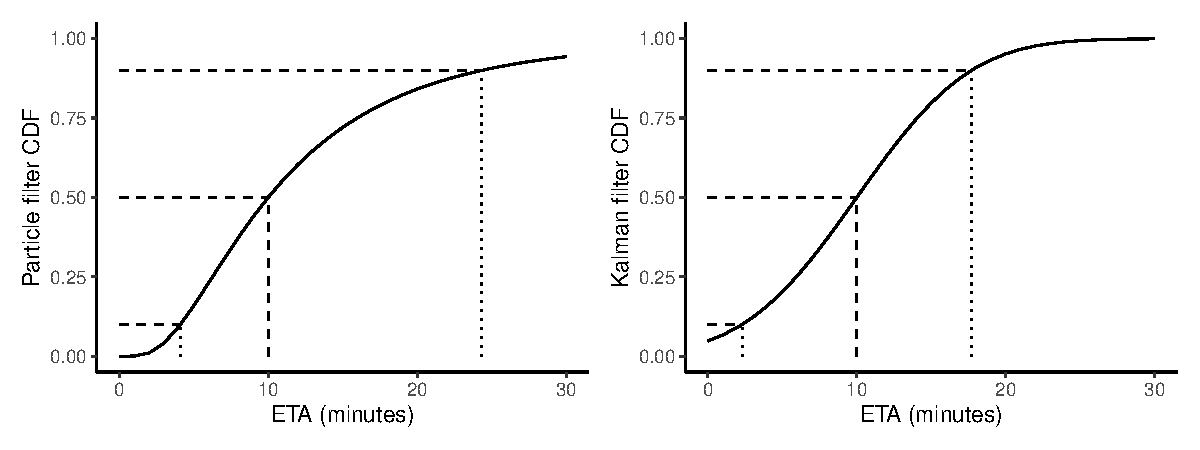
\includegraphics[width=\textwidth]{figure/eta_dist_skew-1} 

}

\caption[Symmetry of arrival time intervals]{Symmetry of arrival time intervals. Symmetric intervals on the probabilty scale map to asymmetric under the particle filter (left), and symmetric intervals under the Kalman filter (right).}\label{fig:eta_dist_skew}
\end{figure}


\end{knitrout}


\begin{knitrout}\small
\definecolor{shadecolor}{rgb}{0.969, 0.969, 0.969}\color{fgcolor}\begin{figure}

{\centering 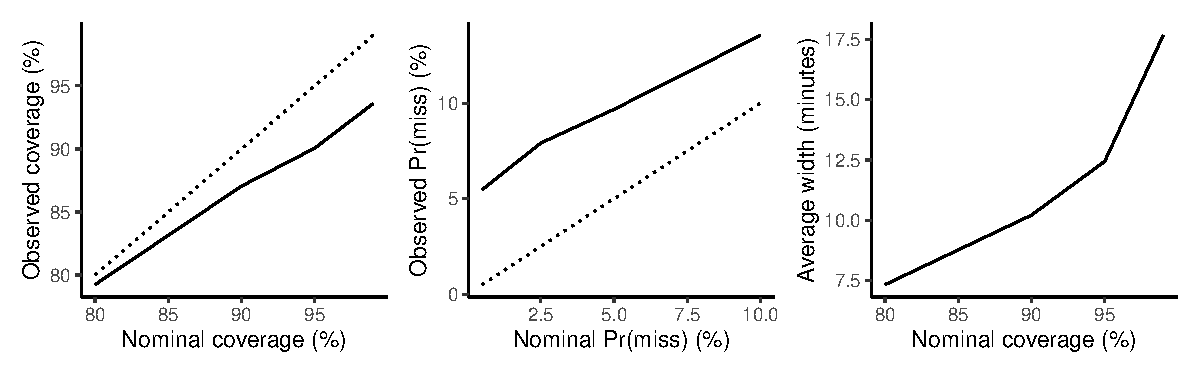
\includegraphics[width=\textwidth]{figure/eta_cis-1} 

}

\caption[ETA CIs]{ETA CIs}\label{fig:eta_cis}
\end{figure}


\end{knitrout}



We computed intervals for $\alpha \in \{0.01, 0.05, 0.1, 0.2\}$, and for each evaluated the observed coverage, the proportion of times that the bus arrived before the lower bound, and the average interval width (in minutes). \Cref{fig:eta_cis} shows that the observed coverage drops slightly as the interval width increases (smaller $\alpha$) and that the probability of the bus arriving before the lower bound is higher than expected, which could indicate that not enough uncertainty is being incorporated. Interval width increases rapidly with coverage probability, demonstrating the trade-off between reliability and usefulness.


Other variables---time until arrival, time of day, or stop sequence---are not considered as we did in the previous chapter, as the results are much the same. However, if desired, such relationships could be explored to choose the best point or interval estimate under any given situation. The goal of this section was to demonstrate that reliability and usefulness can be improved upon by using prediction intervals.

\begin{itemize}
\item I think I might need more discussion here ...
\end{itemize}


\section{Journey planning}
\label{sec:etas-journey-planning}



So far we have been concerned with the arrival time for a bus at a single stop with no consideration of the passenger's commute as a whole. The most straightforward journey consists of a single route choice, so the only decision is which trip to catch; a slightly more complex journey may offer two alternative routes (\cref{sec:journey_simple}) between which the passenger may choose. Finally, there may be no single route which goes from the passenger's start location to their destination, in which case a transfer between two (or more) different routes, or \emph{legs}, is necessary (\cref{sec:journey_transfer}).


Dynamic routing---the selection of candidate trips and real-time assessment of which is \emph{optimal}---is in itself a difficult problem to solve \citep{Hame_2013a,Hame_2013b,Zheng_2016}. There also exist implementations which can take a probabilistic model of arrival time (such as we can obtain by \glspl{cdf}) as input to determine the optimal route (including the selection of candidate routes), such as proposed by \citet{Berczi_2017}. Therefore, for this section we only consider choosing between pre-selected candidate journey options using the arrival time \glspl{cdf} obtained using our \pf{} model. These are compared to the results one might obtain using the currently deployed schedule-delay predictions, which only provide a binary (`Yes' or `No') prediction.


\begin{knitrout}\small
\definecolor{shadecolor}{rgb}{0.969, 0.969, 0.969}\color{fgcolor}\begin{figure}

{\centering 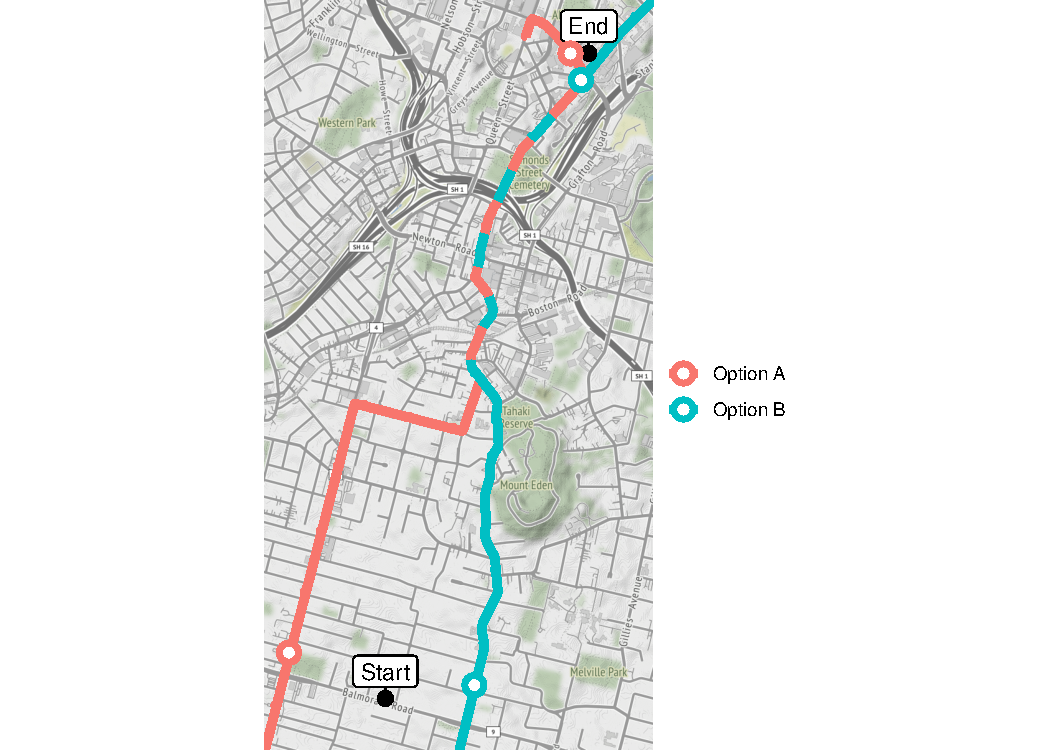
\includegraphics[width=\textwidth]{figure/eta_journey_arrival_prep-1} 

}

\caption[Route options]{Route options}\label{fig:eta_journey_arrival_prep}
\end{figure}


\end{knitrout}

\subsection{Choosing between two alternative routes}
\label{sec:journey_simple}

In this scenario, a passenger lives within walking distance of two major roads, along which various routes travel into the central city, as displayed in \cref{fig:eta_journey_arrival_prep}. The passenger needs to decide which route option to take before leaving home and let's say they have an appointment in town at  2:00~pm. At  1:20~pm, they consult the real-time app on their phone before deciding whether to walk to route option A or B. Factors that could influence their decision include:
\begin{itemize}
\item how long they will have to wait for the next bus;
\item the probability that they will arrive in time for the next bus, and how long until the bus after it;
\item the probability of arriving at their destination on-time, and how early they will be; and
\item the overall length of the journey.
\end{itemize}
We can provide information relating to these questions using the \glspl{cdf} of arrival time at the start and end stops. Walking times at either end of the journey can also be accounted for.


\begin{knitrout}\small
\definecolor{shadecolor}{rgb}{0.969, 0.969, 0.969}\color{fgcolor}\begin{figure}

{\centering 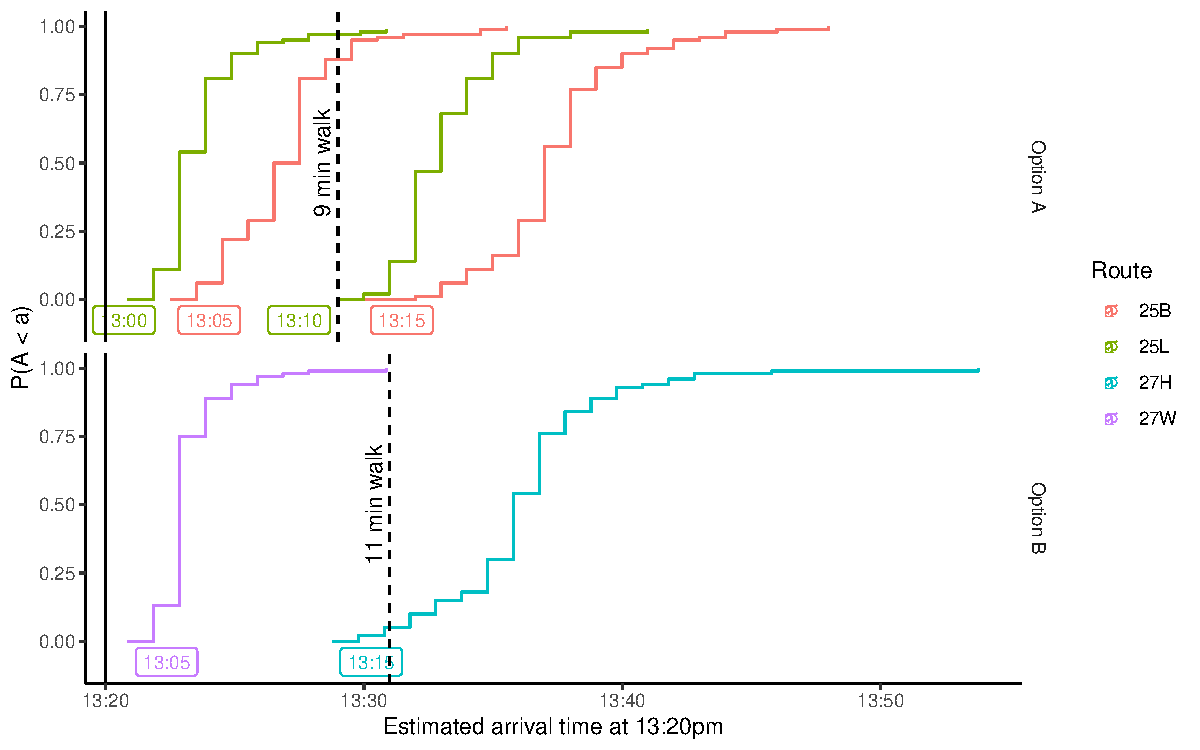
\includegraphics[width=\textwidth]{figure/eta_journey_arrival-1} 

}

\caption[ETA predictions for two route options]{ETA predictions for two route options. The coloured curves represent the CDF of arrival time for individual trips made at 7~am. The vertical black lines indicate the estimated walking time (according to Google Maps) from the Start location to each stop.}\label{fig:eta_journey_arrival}
\end{figure}


\end{knitrout}



\Cref{fig:eta_journey_arrival} displays the \glspl{cdf} of all active trips\footnote{Our application currently only estimates arrival times for active trips.} along the two route options at  1:20~pm when the passenger is about to leave home (solid line), with dashed lines representing the passenger's arrival time at the stops (accounting for walking time). Below each \gls{cdf}, which are coloured by route number, is a label indicating the trip's start time, which is the simplest method of identifying trips. For option A, there appears to be a minimal chance of catching the 1:05~pm 25B, but a good chance of catching the 1:10~pm 25L, with the additional safety of another 25B not long after. As for option B, there is a slightly smaller chance of catching the 1:15~pm 27H, but if missed, it is unclear how long the wait for the next but will be.


\begin{knitrout}\small
\definecolor{shadecolor}{rgb}{0.969, 0.969, 0.969}\color{fgcolor}\begin{figure}

{\centering 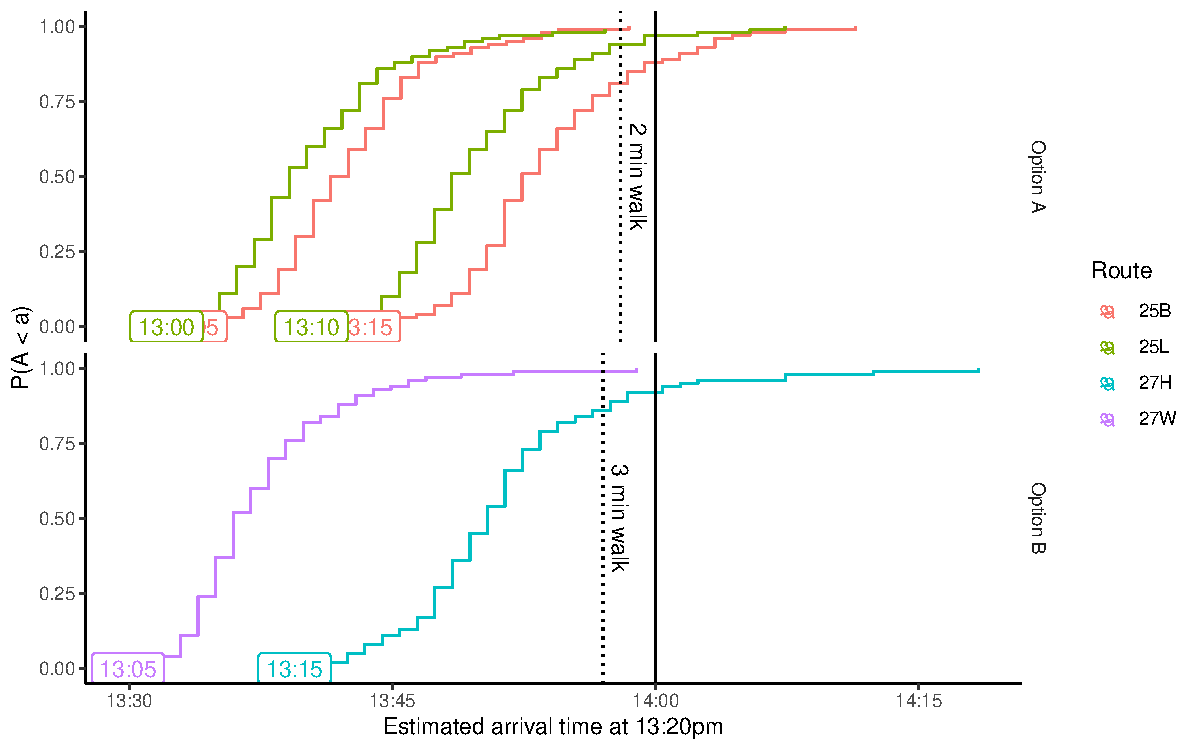
\includegraphics[width=\textwidth]{figure/eta_journey_arriveby-1} 

}

\caption[ETA predictions for two route options]{ETA predictions for two route options. The coloured curves represent the CDF of arrival time for individual trips made at 7~am. The vertical black lines indicate the estimated walking time (according to Google Maps) from the Start location to each stop.}\label{fig:eta_journey_arriveby}
\end{figure}


\end{knitrout}

Based on the arrival results alone, I would choose to walk to option A as it has a good chance of a short wait time; however, the passenger also needs to consider their appointment at 9~am. \Cref{fig:eta_journey_arriveby} provides \glspl{cdf} of each trip's arrival time at the final stop, as well as vertical lines representing the appointment time (solid) and necessary arrival time to allow for walking time (dotted). None of the trips show definitive signs of being late, although the passenger would likely hope to catch the 1:10~pm 25L to maximise their chances of arriving on-time.


\begin{knitrout}\small
\definecolor{shadecolor}{rgb}{0.969, 0.969, 0.969}\color{fgcolor}\begin{table}

\caption{\label{tab:eta_journey_results}Journey planning.}
\centering
\fontsize{8}{10}\selectfont
\begin{tabular}[t]{lllrrllll}
\toprule
\multicolumn{1}{c}{} & \multicolumn{1}{c}{} & \multicolumn{1}{c}{} & \multicolumn{2}{c}{Particle filter} & \multicolumn{2}{c}{GTFS} & \multicolumn{2}{c}{Outcome} \\
\cmidrule(l{3pt}r{3pt}){4-5} \cmidrule(l{3pt}r{3pt}){6-7} \cmidrule(l{3pt}r{3pt}){8-9}
Option & Route & Trip & $P_\text{catch}$ & $P_\text{arrive}$ & Catch & Arrive & Caught & Arrived\\
\midrule
A & 25L & 13:00 & 0.02 & 0.99 & N & Y & N & Y\\
 & 25B & 13:05 & 0.05 & 0.99 & N & Y & N & Y\\
 & 25L & 13:10 & 0.98 & 0.94 & Y & Y & Y & Y\\
 & 25B & 13:15 & 1.00 & 0.81 & Y & N & Y & Y\\
\midrule
B & 27W & 13:05 & 0.00 & 0.99 & N & Y & N & Y\\
 & 27H & 13:15 & 0.90 & 0.86 & Y & Y & Y & Y\\
\bottomrule
\end{tabular}
\end{table}


\end{knitrout}


The \glspl{cdf} allow easy calculation of the predicted probability of success in each scenario, displayed in \cref{tab:eta_journey_results}. Additionally, the binary (`Yes' or `No') predictions made using the schedule-delay method are displayed for comparison, as well as the eventual outcome. That is, would the passenger have caught the bus and did it arrive on time? All of the predictions based on the \pf{} arrival time \glspl{cdf} are valid: small probabilities had a negative outcome, while large probabilities (>0.8) had a positive one. However, the schedule-delay predictions had one incorrect prediction for the arrival of the 1:15~pm 25B at the destination on time; our method predicted an 81\% chance of success for this route.


\begin{knitrout}\small
\definecolor{shadecolor}{rgb}{0.969, 0.969, 0.969}\color{fgcolor}\begin{figure}

{\centering 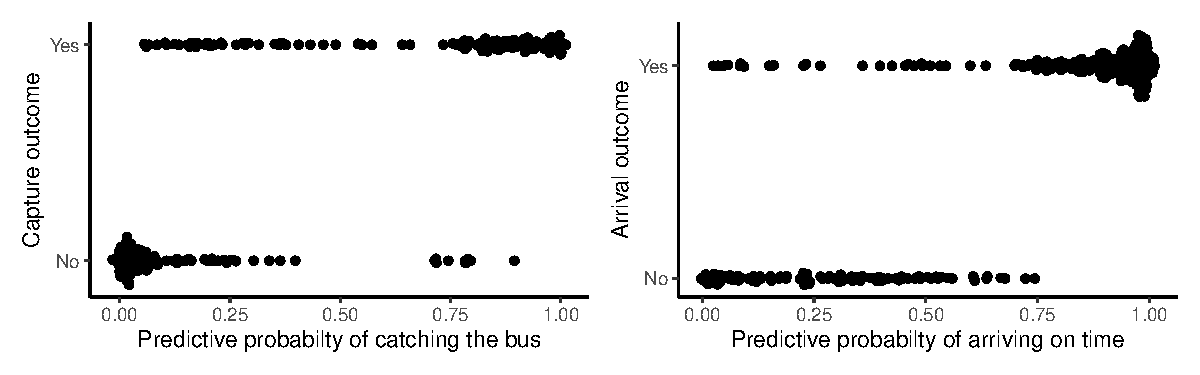
\includegraphics[width=\textwidth]{figure/eta_journey_results_avg-1} 

}

\caption[Results of performing the same journey planning prediction with different starting times (from  9:00~am to  3:00~pm), using the same start and end locations]{Results of performing the same journey planning prediction with different starting times (from  9:00~am to  3:00~pm), using the same start and end locations. Observations are whether or not the passenger would have arrived at the stop before the bus, jittered to better see each observation. Predictive probabilities of 0 and 1 that were correctly estimated have been removed.}\label{fig:eta_journey_results_avg}
\end{figure}

\begin{table}

\caption{\label{tab:eta_journey_results_avg}GTFS prediction results over all journeys, with the displayed values representing the proportion of outcomes in each cell (rows are conditioned by the GTFS prediction of Yes or No. }
\centering
\fontsize{8}{10}\selectfont
\begin{tabular}[t]{llllll}
\toprule
\multicolumn{1}{c}{} & \multicolumn{5}{c}{Observed outcome} \\
\cmidrule(l{3pt}r{3pt}){2-6}
\multicolumn{1}{c}{ } & \multicolumn{2}{c}{Catch bus} & \multicolumn{1}{c}{} & \multicolumn{2}{c}{Arrive on time} \\
\cmidrule(l{3pt}r{3pt}){2-3} \cmidrule(l{3pt}r{3pt}){5-6}
GTS Prediction & No & Yes &  & No & Yes\\
\midrule
No & 0.98 & 0.02 &  & 0.78 & 0.22\\
Yes & 0.09 & 0.91 &  & 0 & 1\\
\bottomrule
\end{tabular}
\end{table}


\end{knitrout}

The results in \cref{fig:eta_journey_arrival,fig:eta_journey_arriveby} and \cref{tab:eta_journey_results} are based on \emph{one single forecast} made at 13h20. To evaluate the overall performance of our prediction method, we repeated the process described above in 5~minute intervals over the off-peak period from  9h00 to 15h00. For the appointment time, we used 30~minute intervals allowing for 15--45 minutes for the journey: leaving between 9h15 and 9h44 had a targetted arrival time of 8h00; 9h45--10h14 targetted 8h30; and so on. The probabilities of catching the bus and arriving on time were calculated for each case. In \cref{fig:eta_journey_results_avg}, we have graphed the distribution of predicted probabilities for each of the two outcomes, for both catching the bus and arriving on time. Only a small number of missed buses had predictions over 50\%, though a larger number of potential buses had low capture probabilities. As for the arrival outcome, successfully arriving on time was usually predicted well, with a small number of low predictions; however, the maximum probability assigned to a failed on-time arrival was 75\%.



For comparison, \cref{tab:eta_journey_results_avg} presents a two-way contingency table for the binary schedule-delay predictions, with the predicted outcomes in rows. In 91\% of the cases where the bus was predicted to arrive after the passenger was the schedule-delay method correct, and 98\% for when it predicted the passenger would miss the bus. For arrival on time, the bus correctly predicted `Yes' 100\% of the time, but only correctly predicted `No' in 78\% of cases. Overall, the schedule-delay method correctly predicted the bus capture in 94\% of cases, and correctly predicted on-time arrival in 89\% of cases.


In both methods, predicting bus capture is more accurate than predicting on-time arrival, since the forecast length is shorter (10~minutes versus 30~minutes). The schedule-delay predictions give a 1-in-10 chance of missing the bus, while our \pf{} provides a less definite prediction (such as 75\%). This opens up the possiblity for passengers to make more informed decisions based on these probabilites and the importance of their constraints, whereas the schedule-delay method can provide, at best, the predicted arrival time as a singular point estimate with no associated uncertainty.





\subsection{Planning a multi-stage journey}
\label{sec:journey_transfer}

A more complex scenario is one in which the passenger must transfer from one route onto another. Transfer journeys are common for travellers commuting from further afield, where there are often several \emph{feeder routes} which connect at a major hub which usually has more frequent trips to another hub. It may also happen that there simply is no single route between a passengers origin and destination, as is demonstrated in \cref{fig:eta_journey_arrival_prep}. In this scenario, the passenger must first catch a bus along route group A\footnote{We use route groups since there are several different routes which make the same journey, as can be seen with route group B in the south-west of \cref{fig:eta_journey_arrival_prep}.} to the stop marked ``Transfer'', at which point they disembark and wait for the next bus along route group B to get to their final destination (marked ``End'').



\begin{knitrout}\small
\definecolor{shadecolor}{rgb}{0.969, 0.969, 0.969}\color{fgcolor}\begin{figure}

{\centering 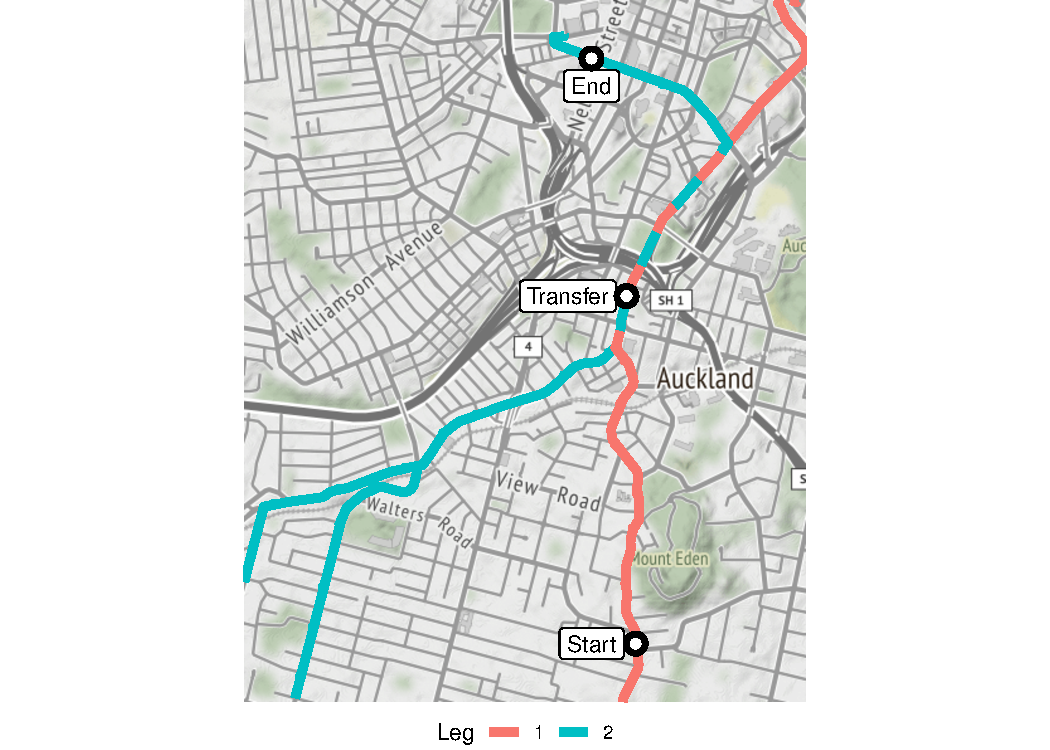
\includegraphics[width=\textwidth]{figure/eta_journey_transfer_prep-1} 

}

\caption[Transfer options]{Transfer options}\label{fig:eta_journey_transfer_prep}
\end{figure}


\end{knitrout}



\begin{knitrout}\small
\definecolor{shadecolor}{rgb}{0.969, 0.969, 0.969}\color{fgcolor}\begin{figure}

{\centering 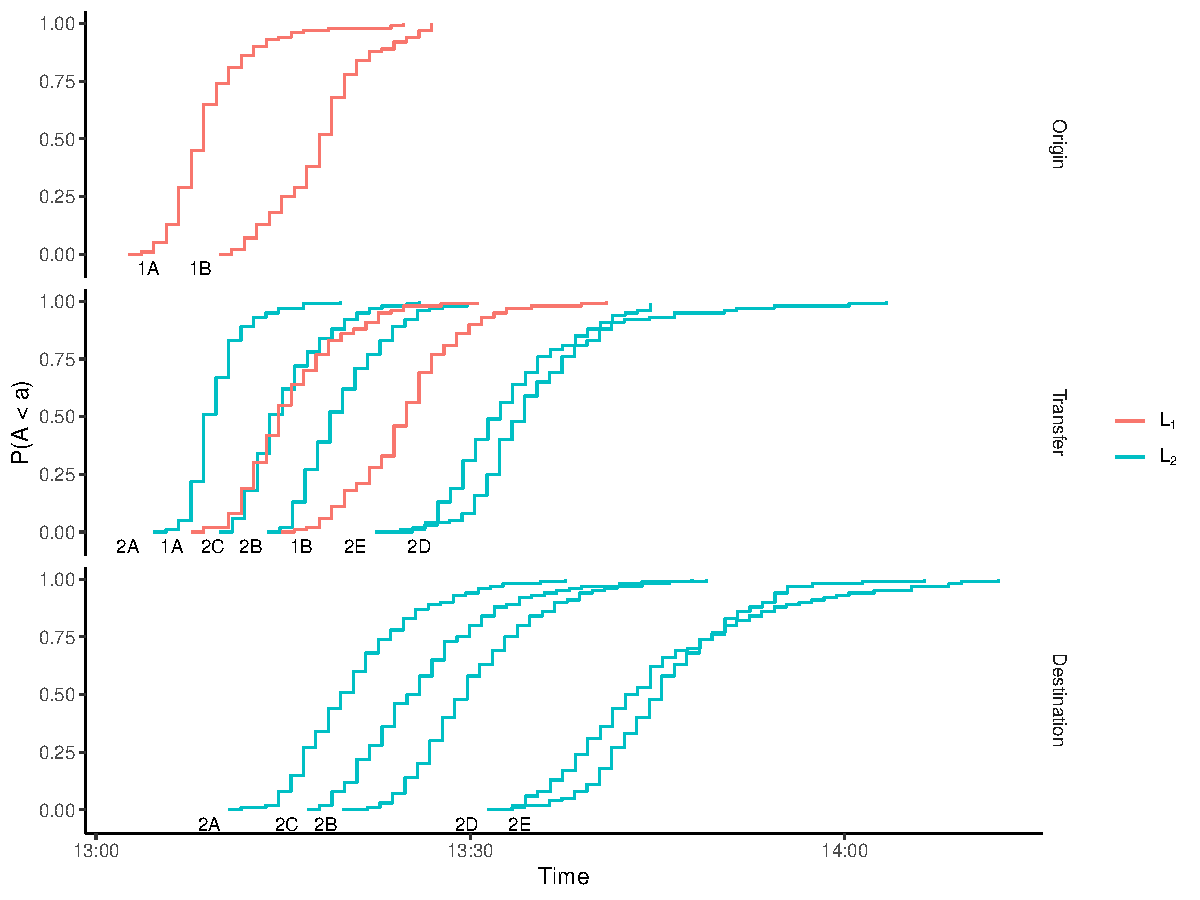
\includegraphics[width=\textwidth]{figure/eta_journey_transfer_graph-1} 

}

\caption[Arrival times]{Arrival times}\label{fig:eta_journey_transfer_graph}
\end{figure}


\end{knitrout}


Similarly to the previous example, we take one single forecast of all trip arrivals at 1~pm to make decisions. Walking time has been removed to simplify the example, but could easily be included if desired. \Cref{fig:eta_journey_transfer_graph} shows, for all active trips at 13h00, their arrival time \glspl{cdf} at the start and transfer stops (for the first leg) and the transfer and end stops (for the second). Additional constraints, such as arrival by a specific time, could of course be added, in this instance we are solely interested in how well a successful transfer can be predicted.


Given \glspl{cdf} for two trips arriving at a stop, the probability that a transfer can successfully be made from A to B can be obtained by the following:
\begin{equation}
\label{eq:eta_total_prob}
\begin{split}
\Pcatch =
\Pr{A < B} &= \sum_{x=1}^{\infty} \Pr{A < B\,|\,B = x}\Pr{B=x} \\
  &= \sum_{x=1}^\infty
    \Pr{A < x} \Pr{B=x} \\
  &= \sum_{x=1}^\infty
    \Pr{A < x} \left[
      \Pr{B < x + 1} - \Pr{B < x}
    \right]
\end{split}
\end{equation}
which we can easily compute given the \glspl{cdf} of the arrival time of each trip obtained from \cref{eq:pf_pdf_arrivaltime}. Table \cref{tab:eta_journey_transfer_res} displays the results, along with the binary predictions using the schedule-delay method along with the observed outcomes. The \pf{} predicts transfer probabilities with reasonable accuracy, with low probabilities resulting in negative outcomes. In contrast, the schedule-delay predicions fail to correctly predict the outcome of a transfer between A1 and B3: it predicts a successful transfer, but infact it is not, while the particle filter predicted a 32\% chance of success. This is where a prediction probability shows its power, in that a passenger could, where applicable, base their decision on how important it is they make the transfer. While this is a fairly non-exciting example (it's a short wait for the next bus), there are other situations where the headway between trips is 30--60~minutes, in which case missing a transfer by a few minutes would be frustrating. However, until our application has been updated to make predictions for upcoming (and not just active) trips, such examples are not yet available.


\begin{knitrout}\small
\definecolor{shadecolor}{rgb}{0.969, 0.969, 0.969}\color{fgcolor}\begin{table}

\caption{\label{tab:eta_journey_transfer_res}Transfer probabilities}
\centering
\fontsize{8}{10}\selectfont
\begin{tabular}[t]{llrll}
\toprule
Leg 1 & Leg 2 & $\mathbb{P}_\text{transfer} & GTFS & Outcome\\
\midrule
1A & 2A & 0.04 & N & N\\
 & 2B & 0.71 & Y & Y\\
 & 2C & 0.32 & Y & N\\
 & 2D & 1.00 & Y & Y\\
 & 2E & 0.99 & Y & Y\\
\midrule
1B & 2A & 0.00 & N & N\\
 & 2B & 0.20 & N & N\\
 & 2C & 0.05 & N & N\\
 & 2D & 0.96 & Y & Y\\
 & 2E & 0.93 & Y & Y\\
\bottomrule
\end{tabular}
\end{table}


\end{knitrout}



\begin{knitrout}\small
\definecolor{shadecolor}{rgb}{0.969, 0.969, 0.969}\color{fgcolor}\begin{figure}

{\centering 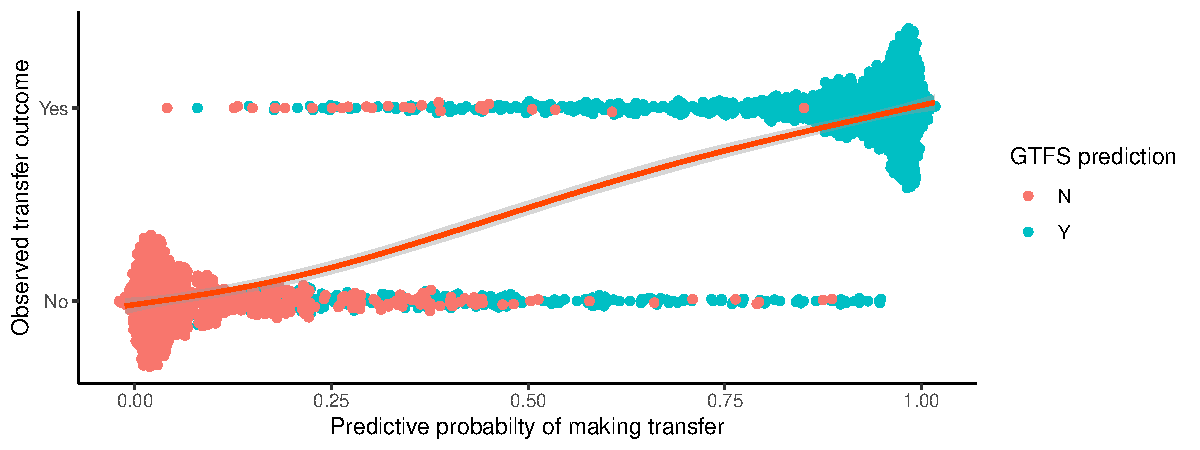
\includegraphics[width=.5\textwidth]{figure/eta_journey_transfer_many-1} 

}

\caption[Results of performing the same transfer journey planning prediction with different starting times (from  9h00 to 15h00)]{Results of performing the same transfer journey planning prediction with different starting times (from  9h00 to 15h00). Observations are whether or not the first bus would arrive at the transfer stop before the second bus, jittered to better see each observation. Additionally, predictive probabilities of 0 and 1 have been removed since, after checking, none or these were invalid and only served to distort the figure.}\label{fig:eta_journey_transfer_many}
\end{figure}

\begin{table}

\caption{\label{tab:eta_journey_transfer_many}Results of running the transfer prediction problem over the course of the day. Rows represent the predicted outcome (No, the transfer will be made, or Yes, it will) and the numbers represent the proportion of predictions with each observed outcome. The GTFS rule is binary, while the particle filter results are based on transfer probability of at least 0.5, 0.8, or 0.95 (as indicated).}
\centering
\fontsize{8}{10}\selectfont
\begin{tabular}[t]{llllllllllll}
\toprule
\multicolumn{1}{c}{} & \multicolumn{11}{c}{Outcome} \\
\cmidrule(l{3pt}r{3pt}){2-12}
\multicolumn{1}{c}{} & \multicolumn{2}{c}{GTFS} & \multicolumn{1}{c}{} & \multicolumn{2}{c}{PF (P > 0.5)} & \multicolumn{1}{c}{} & \multicolumn{2}{c}{PF (P > 0.8)} & \multicolumn{1}{c}{} & \multicolumn{2}{c}{PF (P > 0.95)} \\
\cmidrule(l{3pt}r{3pt}){2-3} \cmidrule(l{3pt}r{3pt}){5-6} \cmidrule(l{3pt}r{3pt}){8-9} \cmidrule(l{3pt}r{3pt}){11-12}
Prediction & No & Yes &  & No & Yes &  & No & Yes &  & No & Yes\\
\midrule
No & 0.97 & 0.03 &  & 0.94 & 0.06 &  & 0.85 & 0.15 &  & 0.7 & 0.3\\
Yes & 0.1 & 0.9 &  & 0.07 & 0.93 &  & 0.03 & 0.97 &  & 0 & 1\\
\bottomrule
\end{tabular}
\end{table}


\end{knitrout}


As before, we proceed to repeat the procedure for multiple times (this time between  9h00 and 15h00), and compute the probabilities of available transfers and whether or not they connected. \Cref{fig:eta_journey_transfer_many} shows the predicted transfer probabilities grouped by outcome, and coloured by the schedule-delay prediction. This is complimented with contingency \cref{tab:eta_journey_transfer_many} for the schedule-delay method and our own, respectively. For the schedule-delay method, in 10\% of cases a predicted successfull connection failed and showed a 3\%, versus only 7\% using the \pf{} with a decision rule of $\Pcatch > 0.5$. The false negative rate was similar for both methods, although slightly higher for our own (6\% versus 3\% for schedule-delay). However, depending on the passenger's requirements, it is possible to reduce the false positive rate under the \pf{} by increasing the threshold. \Cref{tab:eta_journey_transfer_many} also shows the results using 0.8 and 0.95 as the decision rule, which result in a 3\% and 0\% false positive rate, respectively, though these result in quite a significant increase in the false negative rate. Again, by providing probabilities the passenger has the option to decide what level of risk they are willing to take.


In this section we have seen that having access to the full distribution of arrival times enables calculation of event probabilities as opposed to binary outcome predictions. This allows for more sophisticated decision making by travellers depending on their own needs, or by journey planning software. A further advantage of using the \pf{} to estimate the \glspl{cdf} is  that any improvements to the vehicle or network models will automatically be integrated into the arrival prediction component, allowing for further improvments.

